\documentclass[11pt]{article}

\usepackage[preprint]{acl}
%\usepackage[review]{acl}


\usepackage{times}
\usepackage{latexsym}
\usepackage[T1]{fontenc}
\usepackage{microtype}
\usepackage{inconsolata}
\usepackage{graphicx}
\usepackage{hyperref}

% Chinese support (XeLaTeX)
\usepackage{fontspec}
\usepackage{xeCJK}
\usepackage{booktabs}
\usepackage{graphicx}
\usepackage{subcaption}
\usepackage{xurl}
% \usepackage[hidelinks]{hyperref}

\usepackage{amsmath}
\usepackage{amssymb}
\usepackage{xcolor}
\usepackage{tikz}
\usetikzlibrary{arrows.meta,positioning}

\setCJKmainfont{Noto Serif CJK TC}

\newcommand{\githubrepo}{https://github.com/076lin/2026-NYCU-Data-Mining-G06-HW2}

% Red markers for values that are still missing. Search "\todo" and "\tbd"
% before submitting; none may remain.
\newcommand{\todo}[1]{\textcolor{red}{[TODO: #1]}}
\newcommand{\tbd}{\textcolor{red}{??}}
\newcommand{\std}[1]{{\scriptsize$\pm$#1}}

\title{
    Finding the Needle in the Flow: \\
    Anomaly Detection Under Extreme Class Imbalance
    \vspace{0.3em}
    {\footnotesize
    \url{\githubrepo}}\\
    \vspace{0.2em}
    \small{Team 6}
}


\author{
  林程亮 \\ \small 112550125
  \And
  林庠安 \\ \small 315551119
  \And
  林景玄 \\ \small 315551127
  \And
  郭佳翰 \\ \small 315551137
  \AND
  林李奕 \\ \small 315553025
  \And
  王裕昕 \\ \small 315554006
  \And
  顏丞硯 \\ \small 315554021
  \And
  林群佑 \\ \small 315554038
}


\begin{document}
\maketitle
\begin{abstract}
Security analysts need intrusion detectors that flag attacks they have never seen without flooding the alert queue. We study this on CIC-IDS2017 (2.83M network flows, tabular data) with a chronological split in which all three test-day attack families are unseen. On one shared split we compare a single-feature threshold, a $k$NN detector fitted on normal traffic only, and supervised XGBoost. $k$NN ranks unseen attacks best (AUROC 0.921, AP 0.798) at a 3.5\% false-positive rate, but at the threshold frozen on validation it catches only 11.7\% of attacks (F1 0.200). The single-feature rule reaches F1 0.510, and every method stays below the trivial rule that flags everything (0.582). Error analysis traces the failure to threshold transfer between attack mixes, to single-flow features, and to 32,314 mislabelled flows that cause 94\% of $k$NN's false positives.
\end{abstract}


\section{Introduction}
\label{sec:introduction}

Network intrusions such as denial-of-service floods, web exploits and botnet traffic disrupt services and expose data. The users of an Intrusion Detection System (IDS) are security analysts: each alert is triaged by a person, who then blocks the source or isolates the host. A missed attack leaves an intrusion running; too many false alerts make analysts ignore the queue.

Signature-based IDSs only catch known attacks, so we ask: \textbf{can an anomaly-based IDS be trained on benign traffic baselines and still reliably identify rare intrusion attempts in realistic, highly imbalanced traffic?} The data are \textbf{tabular}: one row of numeric statistics per network flow. An \emph{anomaly} is a flow produced by an attack tool. For example, a normal HTTPS flow lasts 115.6\,s and returns 4,863\,B in 18 packets; a PortScan flow lasts 102\,$\mu$s and returns one 6-B packet.

Our contributions are empirical:
\begin{itemize}
\setlength{\itemsep}{0em}
\item A leakage-controlled benchmark in which every test attack family is unseen, with three tiers on one shared split (\S\ref{sec:setup}).
\item Evidence that the normal-only detector ranks unseen attacks best but fails at a frozen threshold, because the threshold does not transfer between attack mixes (\S\ref{sec:results}).
\item An error analysis that explains why a one-feature rule wins on F1, shows a blind spot shared by all tiers, and links 94\% of $k$NN's false positives to label errors (\S\ref{sec:analysis}).
\end{itemize}

\section{Related Work}
\label{sec:related_work}

\citet{sharafaldin2018} introduced CIC-IDS2017 and \citet{maseer2021} benchmarked classical and deep models on it; both evaluate multi-class classifiers on attack types that also appear in training. \citet{engelen2021} found labelling and flow-construction errors in the dataset. \citet{sommer2010} argued that such closed-world results do not carry over to new attacks. Closest to us, \citet{xu2025} hold out three attack types and find that supervised models lose recall on them while one-class models keep it (Table~\ref{tab:related}).

\begin{table}[t]
\centering
\small
\setlength{\tabcolsep}{3pt}
\resizebox{\columnwidth}{!}{%
\begin{tabular}{llll}
\toprule
Work & Task & Paradigm & Test attacks \\
\midrule
\citet{sharafaldin2018} & multi-class & supervised & seen \\
\citet{maseer2021} & multi-class & supervised & seen \\
\citet{xu2025} & binary & sup.\ and one-class & 3 held out, balanced test \\
Ours & binary & normal-only vs.\ sup. & all unseen, real ratio \\
\bottomrule
\end{tabular}}
\caption{Settings on CIC-IDS2017. Results on different splits are context, not a direct comparison.}
\label{tab:related}
\end{table}

\textbf{Positioning.} We differ in the split (chronological, so no test family is seen), in keeping the test set's real class ratio, and in freezing the threshold on validation. Each tier rests on one assumption: Tier~1 assumes that one feature's distance from its normal median signals an attack; Tier~2 ($k$NN) assumes that attacks lie far from normal flows; Tier~3 (XGBoost) assumes that future attacks resemble labelled ones.

\section{Task Definition \& Data}
\label{sec:task_def}

We use the \href{https://www.unb.ca/cic/datasets/ids-2017.html}{CIC-IDS2017 dataset} \citep{sharafaldin2018}: five days of traffic from one test network, exported as flow records. The unit of detection is one flow $\mathbf{x}_i \in \mathbb{R}^{d}$ with label
\begin{equation}
y_i =
\begin{cases}
0, & \text{benign traffic},\\
1, & \text{malicious traffic}.
\end{cases}
\end{equation}
The dataset authors labelled flows from the attack schedule and the attacker's address; every non-BENIGN category is an anomaly. The data hold $N=2{,}830{,}743$ flows, of which 557,646 (19.7\%) are attacks, and $d=57$ features after preprocessing. Labels are noisy: \citet{engelen2021} report mislabelled attack flows, which we quantify in \S\ref{sec:results}.

\begin{table}[t]
\centering
\small
\setlength{\tabcolsep}{3pt}
\resizebox{\columnwidth}{!}{%
\begin{tabular}{lrrrl}
\toprule
Split (period) & Flows & Attacks & \% & Attack families \\
\midrule
Train (Mon--Wed 11:07) & 1,362,859 & 256,198 & 18.80 & Hulk, slowloris, Slowhttptest, FTP/SSH-Patator \\
Val (Wed 11:08--Thu) & 764,639 & 12,525 & 1.64 & GoldenEye, Web $\times$3, Infiltration, Heartbleed \\
Test (Fri) & 703,245 & 288,923 & 41.08 & Bot, PortScan, DDoS \\
\bottomrule
\end{tabular}}
\caption{Chronological split shared by all tiers. Validation also holds 5 slowloris flows.}
\label{tab:split}
\end{table}

\textbf{Split.} To test detection of unseen attacks we split by time (Table~\ref{tab:split}). No test family appears in training or validation. Tier~1 and Tier~2 use normal flows only (semi-supervised); Tier~3 is supervised.

\textbf{Class imbalance.} Validation has 1.64\% attacks (1\,:\,60). ``Always normal'' gives 98.4\% accuracy there and detects nothing, so accuracy is never a main metric. The attack rate also rises to 41.08\% on the test day, which shifts every prevalence-dependent metric.

\section{Exploratory Feature Analysis}
\label{sec:eda}

All statistics in this section use the training split only.

\begin{figure}[t]
\centering
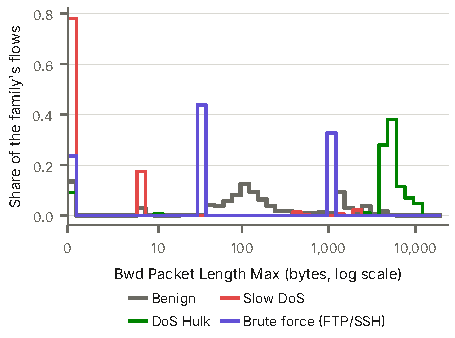
\includegraphics[width=\columnwidth]{fig_eda_feature.pdf}
\caption{Bwd Packet Length Max in the training split. Attack families sit at both extremes of the benign range.}
\label{fig:eda}
\end{figure}

\textbf{Separability.} For each feature we computed the Kolmogorov--Smirnov (KS) distance between benign flows and each of the five training attack types. Bwd Packet Length Max, the largest packet sent back to the initiator, has the highest mean KS (0.803; lowest type 0.727). Figure~\ref{fig:eda} shows why: attacks return either nothing or very large packets, while benign flows centre near 100\,B. The next four features by KS are other backward-size statistics with Spearman $\rho\ge0.90$ to it, so they add little.

\textbf{Structure of normal traffic.} A PCA of normal training flows puts 71\% of the variance on Idle/Active time and 15\% on packet size, and normal flows form separate groups (Figure~\ref{fig:error}a). Training attacks do not share one location: 54\% of Hulk, 37\% of slow-DoS and 71\% of brute-force flows fall inside the region that holds 95\% of normal flows.

\textbf{Preprocessing decisions.} We removed six TCP set-up columns that identified the attacker's host, ten constant and four duplicate columns; heavy tails motivated a signed log transform.

\textbf{Hypotheses.} \textbf{H1}: a two-sided threshold on one response-size feature is a strong naive baseline. \textbf{H2}: unseen attacks lie far from normal flows, so a distance-to-normal score ranks them above benign traffic without labels. \textbf{H3}: attack families occupy different regions, so a threshold tuned on one mix may not transfer to another.

\section{Method}
\label{sec:method}

\begin{figure*}[t]
\centering
\resizebox{\textwidth}{!}{%
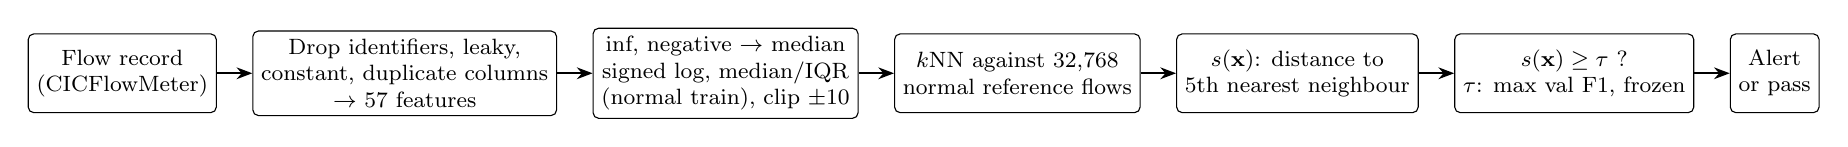
\begin{tikzpicture}[node distance=4.5mm, every node/.style={font=\footnotesize},
  box/.style={draw, rounded corners=2pt, align=center, minimum height=10mm, inner sep=3pt},
  arr/.style={-{Stealth[length=2mm]}, semithick}]
\node[box] (in) {Flow record\\(CICFlowMeter)};
\node[box, right=of in] (sel) {Drop identifiers, leaky,\\constant, duplicate columns\\$\rightarrow$ 57 features};
\node[box, right=of sel] (scale) {inf, negative $\rightarrow$ median\\signed log, median/IQR\\(normal train), clip $\pm10$};
\node[box, right=of scale] (knn) {$k$NN against 32,768\\normal reference flows};
\node[box, right=of knn] (score) {$s(\mathbf{x})$: distance to\\5th nearest neighbour};
\node[box, right=of score] (tau) {$s(\mathbf{x})\ge\tau$ ?\\$\tau$: max val F1, frozen};
\node[box, right=of tau] (out) {Alert\\or pass};
\draw[arr] (in)--(sel); \draw[arr] (sel)--(scale); \draw[arr] (scale)--(knn);
\draw[arr] (knn)--(score); \draw[arr] (score)--(tau); \draw[arr] (tau)--(out);
\end{tikzpicture}}
\caption{Pipeline of the primary method (Tier~2). Scaling parameters and reference flows come from normal training traffic only.}
\label{fig:pipeline}
\end{figure*}

\textbf{Preprocessing.} Infinite and negative values become missing. Each feature is transformed as
\begin{equation}
\tilde{x}_j=\operatorname{clip}\!\Big(\frac{\operatorname{slog}(x_j)-m_j}{\mathrm{IQR}_j},-10,10\Big),
\end{equation}
where $\operatorname{slog}(x)=\operatorname{sign}(x)\log(1+|x|)$ and $m_j$, $\mathrm{IQR}_j$ are the median and interquartile range of deduplicated normal training flows. Missing values take the median.

\textbf{Tier~2: $k$NN (primary).} Let $R$ be 32,768 normal training flows drawn at random. The score is the Euclidean distance to the $k$-th nearest reference flow,
\begin{equation}
s(\mathbf{x})=\lVert\tilde{\mathbf{x}}-\mathbf{r}_{(k)}(\tilde{\mathbf{x}})\rVert_2,\qquad k=5 .
\end{equation}
$k$NN suits tabular data whose normal class is multi-modal (\S\ref{sec:eda}) and needs no training. Figure~\ref{fig:pipeline} shows the pipeline.

\textbf{Tier~1.} $s(\mathbf{x})=|\tilde{x}_j|$ for $j=$ Bwd Packet Length Max, chosen by training KS (\S\ref{sec:eda}). \textbf{Tier~3.} $s(\mathbf{x})$ is the attack probability of XGBoost trained on labelled training flows, with benign and attack flows weighted equally and the five attack types weighted equally within attacks.

\textbf{Threshold.} For every tier, $\tau$ maximises F1 on validation and is then frozen; a flow is flagged when $s(\mathbf{x})\ge\tau$. The test set is never used.

\textbf{Cost of errors.} A false positive costs analyst time; a false negative leaves an intrusion undetected. At 1.64\% prevalence, maximising F1 requires high precision, so our $\tau$ suppresses false positives (validation FPR 0.26\% for Tier~2) at the price of missed attacks.

\section{Experimental Setup}
\label{sec:setup}

\textbf{Split and leakage control.} Train, validation and test hold 48.1\%, 27.0\% and 24.8\% of the flows in time order, with fixed indices shared by all tiers. Identifiers (addresses, ports, protocol, timestamp) are never inputs. Constant and duplicate columns, scaling parameters and medians are fitted on training data only. Duplicates are removed from training only. One-class tiers see normal training flows only; validation labels are used only for $\tau$ and model selection. Each frozen configuration was evaluated on the test set once.

\textbf{Configurations.} Tier~2: $k=5$, $|R|=32{,}768$, three seeds that draw different reference sets; PyTorch 2.5.1 on one RTX~3080. Tier~3: XGBoost 3.4.1 (\texttt{hist}) on an Apple M5; 80\% of training for fitting and a stratified 20\% holdout for early stopping (50 rounds, weighted log loss) and a grid over depth $\{4,6,8\}$ and learning rate $\{0.05,0.1\}$; selected depth 4 and rate 0.1 with about 524 trees; three seeds. Tier~1 is deterministic.

\textbf{Metrics.} Average precision (AP) and AUROC measure ranking without a threshold; AP reflects the analyst's precision under imbalance. F1, recall and false-positive rate (FPR) at the frozen $\tau$ describe the deployed operating point: recall is the share of intrusions caught and FPR drives the alert volume. We report mean $\pm$ sample std over three seeds, and test differences with a one-sample $t$-test (against deterministic Tier~1) or Welch's $t$-test.

\section{Results}
\label{sec:results}

\subsection{Main Results}

\begin{table*}[t]
\centering
\small
\setlength{\tabcolsep}{4.2pt}
\resizebox{\textwidth}{!}{%
\begin{tabular}{l cc ccccc cc}
\toprule
 & \multicolumn{2}{c}{Validation (1.64\% attacks)} & \multicolumn{5}{c}{Friday test (41.08\% attacks)} & \multicolumn{2}{c}{Cost} \\
\cmidrule(lr){2-3}\cmidrule(lr){4-8}\cmidrule(lr){9-10}
Method & AP & F1@$\tau$ & AP & AUROC & F1@$\tau$ & Recall@$\tau$ & FPR@$\tau$ (\%) & Fit (s) & ms\,/\,flow \\
\midrule
\textit{Flag every flow} & \textit{0.016} & \textit{0.032} & \textit{0.411} & \textit{0.500} & \textit{0.582} & \textit{1.000} & \textit{100} & -- & -- \\
T1 $\cdot$ single feature & 0.036 & 0.103 & 0.577 & 0.762 & \textbf{0.510} & \textbf{0.443} & 20.54 & 0 & $2.4{\times}10^{-5}$ \\
T2 $\cdot$ $k$NN (ours) & \textbf{0.449}\std{0.036} & \textbf{0.653}\std{0.010} & \textbf{0.798}\std{0.023} & \textbf{0.921}\std{0.003} & 0.200\std{0.042} & 0.117\std{0.029} & \textbf{3.48}\std{1.20} & 0 & $3.0{\times}10^{-3}$ \\
T3 $\cdot$ XGBoost (sup.) & 0.119\std{0.005} & 0.270\std{0.005} & 0.782\std{0.008} & 0.858\std{0.006} & 0.431\std{0.010} & 0.297\std{0.010} & 5.56\std{0.39} & 27.1\std{2.3} & $5.3{\times}10^{-4}$ \\
\bottomrule
\end{tabular}}
\caption{Main results on the shared split (mean $\pm$ sample std over 3 seeds; Tier~1 is deterministic). Bold marks the best tier per column (lowest for FPR); the italic row is the trivial rule. Latency is batch time per flow (Tier~1 on CPU, Tier~2 on GPU with 170\,MiB peak memory, Tier~3 on an Apple M5). Tier~1 and Tier~2 fit no weights.}
\label{tab:main}
\end{table*}

\textbf{At the frozen threshold, Tier~1 wins} (Table~\ref{tab:main}). Its test F1 is 0.510, against 0.431 for Tier~3 and 0.200 for Tier~2; both gaps to Tier~1 are far outside seed variation (one-sample $t(2)=-13.6$ and $-12.7$; $p=0.005$ and $0.006$). Yet no tier beats flagging every flow (0.582): at 41\% attacks, F1 rewards alert volume, and Tier~1 alerts on 30.3\% of flows.

\textbf{As a ranker, Tier~2 wins}, which supports H2. Its AUROC exceeds Tier~3's by 0.063 (Welch $t=16.4$, $p<0.001$), but its AP gap (0.016) is inside seed std ($t=1.19$, $p=0.34$), so on AP we claim ``comparable''. Compared post hoc at Tier~1's FPR, Tier~2 catches 99.4\% of attacks, Tier~3 71.2\% and Tier~1 44.3\%; its best F1 in hindsight is 0.91.

\textbf{Why Tier~2 loses at $\tau$.} 82\% of validation attacks are GoldenEye, which lies far from normal traffic, so max-F1 picks a strict $\tau$. On Friday that $\tau$ sits above almost every new attack. A Shapley decomposition of the F1 change ($0.653\rightarrow0.200$) attributes $-0.447$ to the change in attack families, $-0.137$ to normal traffic and $+0.131$ to prevalence. This confirms H3.

\textbf{Why Tier~3 does not beat Tier~2.} Supervision covers five attack types, so Tier~3 detects a new attack only if it resembles one of them \citep{sommer2010}: its AP is 1.000 on held-out flows of seen types and 0.782 on Friday. \citet{xu2025} report the same loss; their one-class models keep recall, ours keeps only ranking.

\textbf{Label errors.} On Friday, 32,314 BENIGN flows run between the victim web server and the attacker's address, 97\% of them inside the DDoS window; such flows are known label errors \citep{engelen2021}. They make up about 94\% of Tier~2's false positives. Excluding them (post hoc) lowers Tier~2's FPR from 3.48\% to 0.20\% and raises its AP from 0.80 to 0.96, while Tier~3's AP moves from 0.782 to 0.799: its training data held 6,583 such flows labelled BENIGN.

\subsection{Controlled Ablations}
\label{sec:ablation}

\begin{table}[t]
\centering
\small
\setlength{\tabcolsep}{4pt}
\resizebox{\columnwidth}{!}{%
\begin{tabular}{llcccc}
\toprule
Factor & Setting & Val AP & $\Delta$ & Val F1@$\tau$ & $\Delta$ \\
\midrule
Full & $k{=}5$, $k$-th dist., 32,768 & 0.452\std{0.057} & -- & 0.650\std{0.005} & -- \\
\midrule
$k$ & 1 & 0.414\std{0.084} & $-0.038$ & 0.571\std{0.103} & $-0.079$ \\
 & 10 & 0.450\std{0.045} & $-0.002$ & 0.632\std{0.003} & $-0.018$ \\
 & 20 & 0.383\std{0.011} & $-0.069$ & 0.586\std{0.009} & $-0.064$ \\
Score & mean of 5 distances & 0.432\std{0.099} & $-0.020$ & 0.602\std{0.084} & $-0.048$ \\
Reference size & 4,096 & 0.381\std{0.046} & $-0.071$ & 0.538\std{0.005} & $-0.112$ \\
 & 16,384 & 0.410\std{0.077} & $-0.042$ & 0.626\std{0.018} & $-0.024$ \\
\bottomrule
\end{tabular}}
\caption{Ablations of Tier~2 on validation (mean $\pm$ std over 3 seeds; one factor changed at a time; $\Delta$ vs.\ the full method). CPU re-run with the same seeds and sampling rule; the reference samples differ slightly from those behind Table~\ref{tab:main}.}
\label{tab:ablation}
\end{table}

Table~\ref{tab:ablation} changes one factor of Tier~2 at a time. The full setting has the best AP and F1. On AP, no change exceeds the seed std (0.057): AP is noisy because one family, GoldenEye, dominates validation. On F1 (seed std 0.005) the effects are clear: 4,096 reference flows cost 0.112 and $k=20$ costs 0.064, both far beyond seed std (paired $t$-test, $p=0.001$ and $p=0.014$); $k=10$ costs 0.018. Two changes give negative results of a different kind: $k=1$ and the mean-of-5 score are unstable across seeds (F1 std 0.103 and 0.084), because they depend on the single nearest neighbour, which changes with the reference sample. Halving the reference set to 16,384 stays within noise ($-0.024$), so the method could run at half the cost.

\section{Analysis}
\label{sec:analysis}

\subsection{Error Analysis}

\begin{figure*}[t]
\centering
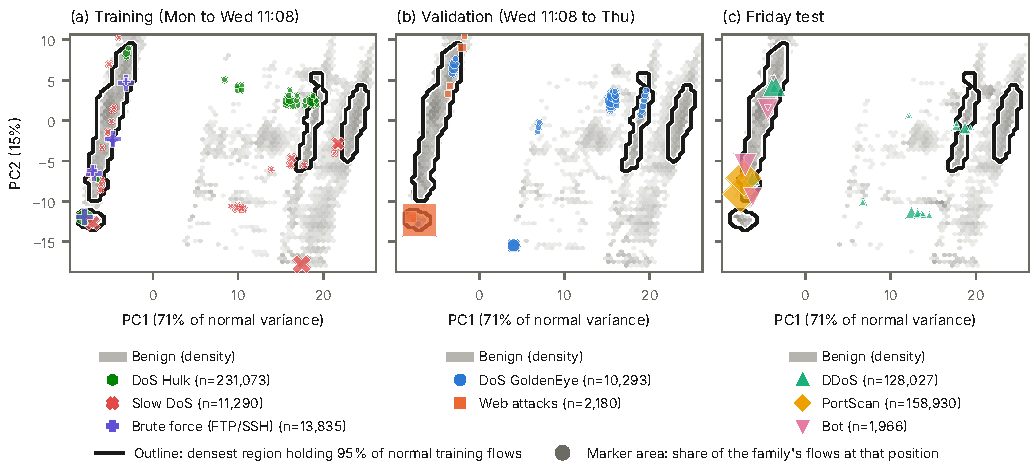
\includegraphics[width=\textwidth]{fig_pca.pdf}
\caption{Flows on the first two principal components of normal training traffic (PCA fitted on normal training flows only). Grey shows benign density; the outline encloses the densest region holding 95\% of normal training flows. For each attack family, marker area is the share of its flows at that position.}
\label{fig:error}
\end{figure*}

\begin{table}[t]
\centering
\small
\setlength{\tabcolsep}{3.2pt}
\resizebox{\columnwidth}{!}{%
\begin{tabular}{l ccc ccc}
\toprule
 & \multicolumn{3}{c}{Recall@$\tau$} & \multicolumn{3}{c}{AUROC} \\
\cmidrule(lr){2-4}\cmidrule(lr){5-7}
Family (share) & T1 & T2 & T3 & T1 & T2 & T3 \\
\midrule
PortScan (55.0\%) & 0.007 & 0.002 & 0.01 & 0.701 & \textbf{0.899} & 0.790 \\
DDoS (44.3\%) & \textbf{0.990} & 0.262 & 0.661 & 0.843 & \textbf{0.952} & -- \\
Bot (0.7\%) & 0.001 & 0.008 & 0.00 & 0.465 & \textbf{0.752} & 0.716 \\
\bottomrule
\end{tabular}}
\caption{Friday results by attack family (AUROC against Friday benign flows).}
\label{tab:family}
\end{table}

\begin{table*}[t]
\centering
\small
\setlength{\tabcolsep}{4pt}
\resizebox{\textwidth}{!}{%
\begin{tabular}{lllrrrrrll}
\toprule
Tier & Type & Label & Row ID & Duration ($\mu$s) & Fwd\,/\,Bwd pkts & Bwd max (B) & $s(x)$ & Largest term of the score & Distance to $\tau$ \\
\midrule
T1 & FP & BENIGN & 2127500 & 113,757,376 & 545\,/\,0 & 0 & 2.412 & the single feature & inversion ($+0.69$) \\
T1 & FN & PortScan & 2357130 & 102 & 1\,/\,1 & 6 & 1.428 & the single feature & inversion ($-0.29$) \\
T1 & FN & Bot & 2183874 & 134,812 & 4\,/\,3 & 128 & 0.045 & the single feature & inversion ($-1.67$) \\
T1 & FP & BENIGN & 2398923 & 5,030,618 & 14\,/\,14 & 3,525 & 1.7174 & the single feature & near miss ($+1.4{\times}10^{-4}$) \\
\midrule
T2 & FN & PortScan & 2454412 & 455 & 2\,/\,1 & 2 & 2.292 & PSH Flag Count (19\%) & inversion \\
T2 & FN & Bot & 2286836 & 1,001,534 & 3\,/\,3 & 6 & 1.686 & Flow IAT Min (95\%) & inversion \\
T2 & FN & DDoS & 2687946 & 10,093,717 & 4\,/\,0 & 0 & 5.0942 & Active Mean/Min/Max (68--88\%) & near miss ($-1.1{\times}10^{-4}$) \\
T2 & TP & DDoS & 2723650 & 5,021,793 & 4\,/\,0 & 0 & 6.462 & Active Mean/Min/Max (68--88\%) & $+1.37$ \\
T2 & FP & BENIGN & 2132365 & 45,670,096 & 6\,/\,0 & 0 & 12.580 & Idle Std (63\%) & $2.5\,\tau$ \\
\bottomrule
\end{tabular}}
\caption{Failure cases on Friday. Tier~1: $\tau=1.717$. Tier~2: seed 20261104, $\tau=5.0943$; percentages are exact shares of $s^2$. Row ID is the position in the shared metadata.}
\label{tab:cases}
\end{table*}

\textbf{Attack families occupy different regions} (Figure~\ref{fig:error}). Only 29\% of GoldenEye flows fall inside the normal outline, so a strict $\tau$ separates them, while 96\% of Web-attack flows are inside. On Friday, 98\% of Bot and 72\% of DDoS flows are inside. The shares outside the outline (GoldenEye 71\%, DDoS 28\%) match Tier~2's recall on these families (68\%, 26\%). Half of the PortScan flows lie just outside the outline, beside the main normal group, yet Tier~2 catches 0.2\%: their nearest training flow is benign for 99\% of samples. Tier~2 ranks PortScan and Bot above most benign flows (Table~\ref{tab:family}), but not above a threshold tuned on GoldenEye.

\textbf{Why the naive baseline wins.} The frozen Tier~1 rule is equivalent to: flag a flow whose largest backward packet is at most 2\,B or at least 3,525\,B. DDoS responses have a median of 5,755\,B against 82\,B for benign flows, so Tier~1 catches 99.0\% of DDoS, which supplies 126,797 of its 127,937 true positives. H1 therefore holds for one family only: Tier~1 wins because one feature matches the family that forms 44\% of Friday attacks. On Bot its AUROC is below chance (0.465): Bot flow \#2183874 (128\,B) sits at the benign median (117\,B).

\textbf{Tier~1 errors.} 99.22\% of PortScan flows have a feature value of exactly 6\,B and score $1.428<\tau$; they are 98\% of Tier~1's false negatives. 47,316 benign flows have the same value, so no threshold on this feature separates them. 92.75\% of its false positives have a value of 0\,B ($s=2.412$): a flow without backward payload is far from the benign median but common in legitimate traffic.

\textbf{Tier~2 cases} (Table~\ref{tab:cases}). DDoS flow \#2687946 misses $\tau$ by $1.1{\times}10^{-4}$ while \#2723650 is caught; both are 4-packet half-open HTTP requests. Benign flow \#2132365 has the highest benign score: a one-class model flags legitimate traffic that training never contained.

\textbf{Tier~3.} Every training attack type has an empty response (median Bwd Packet Length Min 0\,B against 48\,B for benign), so XGBoost learns the shortcut ``no response payload means attack'' \citep{geirhos2020}. PortScan and Bot reply with 6\,B and are passed.

\textbf{Shared blind spot and first fix.} All tiers score one flow at a time, but PortScan and Bot are anomalous only in context (one source probing many ports; periodic beaconing). 99.1\% of PortScan flows carry at most one packet per direction, as do 20.6\% of benign flows. The first fix is per-source windowed features (e.g.\ distinct destination ports within 60\,s), not a larger model.

\subsection{Practical Impact and Interpretability}

\textbf{Practical impact.} At validation's realistic attack rate, Tier~1 raises 208,642 alerts with 17.3 false alarms per detected attack, which no analyst team can review; Tier~2 raises 8,993 alerts with 0.28. On Friday Tier~2 stays quiet (FPR 3.48\%) but misses 88\% of attacks. For analysts, Tier~2 at the frozen $\tau$ is a low-noise detector of volumetric DoS, not a general intrusion detector.

\textbf{Interpretability.} The squared $k$NN score is a sum of per-feature terms, so each feature's share is exact (Table~\ref{tab:cases}). Timing features are the largest term in four of the five Tier~2 cases. For the two DDoS flows, Active Mean/Min/Max carries 68--88\% of the distance and decides which one crosses $\tau$; the missing response does not. An analyst cannot act on an explanation that describes timing jitter rather than attack behaviour. Tier~3's explanations mislead on new attacks: the mean SHAP value \citep{lundberg2017} of Bwd Packet Length Min is $-2.74$ for PortScan.

\section{Conclusion \& Limitations}
\label{sec:conclusion}

\textbf{Key findings.} Can an IDS trained on benign traffic reliably identify rare intrusions? Only in part. The normal-only $k$NN ranks three unseen attack families best (AUROC 0.921), and at a 1.64\% attack rate it reaches F1 0.653 with a 0.26\% false-positive rate. It is not reliable at a fixed threshold: on Friday it catches 11.7\% of attacks (F1 0.200), below a one-feature rule (0.510) and below flagging everything (0.582).

\textbf{Reflection and next steps.} The threshold rule mattered more than any model setting in Table~\ref{tab:ablation}. Starting again, we would set $\tau$ by alert budget on benign validation traffic. Next steps: (1) per-source windowed features for PortScan and Bot; (2) relabelling victim-to-attacker flows before training and evaluation.

\textbf{Limitations.} The data cover five days of one test network from 2017; each attack family appears in one time window, so family and day are confounded. Matched-FPR, hindsight and label-exclusion results use Friday labels and are diagnostic only.

\textbf{Deployment.} Normal traffic drifts, so the reference set needs periodic refresh and the alert rate needs monitoring. Latency is far below a millisecond, but a flow record exists only when the flow ends. Inputs exclude addresses and ports, which limits privacy exposure.


\section*{Contributions of Each Member}

\begin{itemize}
\setlength{\itemsep}{0em}
\setlength{\parsep}{0em}
\item \mbox{林程亮(112550125):} \todo{tasks}
\item \mbox{林庠安(315551119):} \todo{tasks}
\item \mbox{林景玄(315551127):} \todo{tasks}
\item \mbox{郭佳翰(315551137):} \todo{tasks}
\item \mbox{林李奕(315553025):} \todo{tasks}
\item \mbox{王裕昕(315554006):} \todo{tasks}
\item \mbox{顏丞硯(315554021):} \todo{tasks}
\item \mbox{林群佑(315554038):} coordination; integration of \S\ref{sec:results}--\S\ref{sec:conclusion}; Figures~\ref{fig:eda} and~\ref{fig:error}. \todo{confirm}
\end{itemize}

\textbf{AI usage.} We used Claude (Anthropic) to draft and edit text, to write the figure and ablation scripts, to run the Tier~2 ablations, and to check numbers against the raw data. \todo{other tools.} Method and experiment design and all conclusions were decided and verified by the team.

\clearpage

% \bibliographystyle{acl_natbib}
\bibliography{custom}
\end{document}
